\section{Jointly Typical Sequence, Jointly Typical Set}
\centerline{Book $\S 7.6$ (P221)}
$$X^n\triangleq \left(X_1,\ldots,X_n\right), Y^n\triangleq \left(Y_1,\ldots,Y_n\right)$$

\begin{definition}
基于joint distribution $P_{X,Y}(x,y)$: $(X_i,Y_i)\stackrel{i.i.d.}{\sim}P_{X,Y}(x,y)$, 产生的 sequence $(X^n,Y^n)$ belongs the $\epsilon$-jointly typical set $A_{\epsilon}^{(n)}(P_{X,Y})$ if
\begin{itemize}
\item[1.] $\left|-\dfrac{1}{n}\log p(X^n)-H(X)\right|<\epsilon$
\item[2.] $\left|-\dfrac{1}{n}\log p(Y^n)-H(Y)\right|<\epsilon$
\item[3.] $\left|-\dfrac{1}{n}\log p(X^n,Y^n)-H(X,Y)\right|<\epsilon$
\end{itemize}
\end{definition}
1. 2. 说明 $X^n,Y^n$分别是typical sequence, 但是无法说明 $(X^n,Y^n)$ 是jointly typical sequence.(推不出3.)

类似于单变量的AEP, 我们可以推演出 Joint AEP:
\begin{proposition}
1. $2^{-n\left(H(X,Y)+\epsilon\right)}\leq p(x^n,y^n)\leq 2^{-n\left(H(X,Y)-\epsilon\right)}$ \\
2. $P\left(\left(x^n,y^n\right)\in A_{\epsilon}^{(n)}(P_{X,Y})\right) \to 1$ as $n\to\infty$. \\
3. $(1-\epsilon)2^{n\left(H(X,Y)-\epsilon\right)}\leq |A_{\epsilon}^{(n)}(P_{X,Y})|\leq 2^{n\left(H(X,Y)+\epsilon\right)}$ \\
4. $P\left[(\tilde{x}^n,\tilde{y}^n)\in A_{\epsilon}^{(n)}(p(x)p(y))\right]\to 2^{-nI(X;Y)}$ \qquad($\tilde{x},\tilde{y}$独立产生)
\end{proposition}

proof: 1. 由定义可得. \\
2. 由 jointly typical set 的定义可得: in probability:
$$-\dfrac{1}{n}\log p(x^n)\to H(X), \quad -\dfrac{1}{n}\log p(y^n)\to H(Y), \quad -\dfrac{1}{n}\log p(x^n,y^n)\to H(X,Y)$$
i.e. $\exists N_1,N_2,N_3\in\mathbb{N}$, s.t.
\begin{align*}
\Pr\left[\left|-\dfrac{1}{n}\log p(x^n)-H(X)\right| \geq \epsilon\right] &< \delta = \dfrac{\epsilon}{3} \text{\qquad for } n\geq N_1 \\
\Pr\left[\left|-\dfrac{1}{n}\log p(y^n)-H(Y)\right| \geq \epsilon\right] &< \delta = \dfrac{\epsilon}{3} \text{\qquad for } n\geq N_2 \\
\Pr\left[\left|-\dfrac{1}{n}\log p(x^n,y^n)-H(X,Y)\right| \geq \epsilon\right] &< \delta = \dfrac{\epsilon}{3} \text{\qquad for } n\geq N_3
\end{align*}
Then let $N=\max\{N_1,N_2,N_3\}$, we have $\forall n\geq N$:
$$p\left(x^n\notin A_{\epsilon}^{(n)}(p_X)\right)<\dfrac{\epsilon}{3}, \quad p\left(y^n\notin A_{\epsilon}^{(n)}(p_Y)\right)<\dfrac{\epsilon}{3}, \quad p\left(x^n,y^n\notin A_{\epsilon}^{(n)}(p_{X,Y})\right)<\dfrac{\epsilon}{3}\Rightarrow$$
\begin{align*}
p\left[\left(x^n,y^n\right)\in A_{\epsilon}^{(n)}(P_{X,Y})\right] &= 1 - p\left[\left(x^n,y^n\right)\notin A_{\epsilon}^{(n)}(P_{X,Y})\right] \\
&\geq 1 - p\left(x^n\notin A_{\epsilon}^{(n)}(P_X)\right) - p\left(y^n\notin A_{\epsilon}^{(n)}(P_Y)\right) \\
&\qquad - p\left(x^n,y^n\notin A_{\epsilon}^{(n)}(P_{X,Y})\right) \text{\qquad (违反 jointly typical set任意一条)} \\
&\geq 1 - \dfrac{\epsilon}{3}\times 3 \\
&= 1 - \epsilon \to 1 \text{\qquad as } n\to\infty
\end{align*}

3. 由2.可得下界:
\begin{align*}
1-\epsilon &\leq p\left[\left(x^n,y^n\right)\in A_{\epsilon}^{(n)}(P_{X,Y})\right] \text{\qquad (由2.可得)}\\
&= \sum_{(x^n,y^n)\in A_{\epsilon}^{(n)}(P_{X,Y})}p(x^n,y^n) \leq \left|A_{\epsilon}^{(n)}(P_{X,Y})\right|2^{-n\left(H(X,Y)-\epsilon\right)}
\end{align*}
i.e. $(1-\epsilon)2^{n\left(H(X,Y)-\epsilon\right)} \leq \left|A_{\epsilon}^{(n)}(P_{X,Y})\right|$ \\
上界:
\begin{align*}
1 &= \sum_{(x^n,y^n)}p(x^n,y^n) \geq \sum_{(x^n,y^n)\in A_{\epsilon}^{(n)}(P_{X,Y})}p(x^n,y^n) \\
&\geq \left|A_{\epsilon}^{(n)}(P_{X,Y})\right|2^{-n\left(H(X,Y)+\epsilon\right)}
\end{align*}
i.e. $\left|A_{\epsilon}^{(n)}(P_{X,Y})\right| \leq 2^{n\left(H(X,Y)+\epsilon\right)}$ \\
结合上下界可得
$$(1-\epsilon)2^{n\left(H(X,Y)-\epsilon\right)} \leq \left|A_{\epsilon}^{(n)}(P_{X,Y})\right| \leq 2^{n\left(H(X,Y)+\epsilon\right)}$$

4. Since $(\tilde{x}^n,\tilde{y}^n)\stackrel{i.i.d.}{\sim} p(x)p(y)$, we have
$$p\left[(\tilde{x}^n,\tilde{y}^n)\in A_{\epsilon}^{(n)}(p(X,Y))\right] = \sum_{(\tilde{x}^n,\tilde{y}^n)\in A_{\epsilon}^{(n)}(p(X,Y))}p(\tilde{x})p(\tilde{y}) = \left|A_{\epsilon}^{(n)}(p(X,Y))\right|p(\tilde{x})p(\tilde{y})$$
结合3. $(1-\epsilon)2^{n\left(H(X,Y)-\epsilon\right)} \leq \left|A_{\epsilon}^{(n)}(P_{X,Y})\right| \leq 2^{n\left(H(X,Y)+\epsilon\right)}$,及 $\tilde{x}^n,\tilde{y}^n$是typical sequence ($2^{-n\left(H(X)+\epsilon\right)}\leq p(\tilde{x}^n)\leq 2^{-n\left(H(X)-\epsilon\right)}$) 可得
\begin{align*}
p\left[(\tilde{x}^n,\tilde{y}^n)\in A_{\epsilon}^{(n)}(p(x)p(y))\right] &\leq 2^{-n\left((H(X)-\epsilon)+(H(Y)-\epsilon)-(H(X,Y)+\epsilon)\right)} = 2^{-n\left(I(X;Y)-3\epsilon\right)} \\
p\left[(\tilde{x}^n,\tilde{y}^n)\in A_{\epsilon}^{(n)}(p(x)p(y))\right] &\geq (1-\epsilon)2^{-n\left((H(X)+\epsilon)+(H(Y)+\epsilon)-(H(X,Y)-\epsilon)\right)} = (1-\epsilon)2^{-n\left(I(X;Y)+3\epsilon\right)}
\end{align*}
合并可得
$$(1-\epsilon)2^{-n\left(I(X;Y)+3\epsilon\right)} \leq p\left[(\tilde{x}^n,\tilde{y}^n)\in A_{\epsilon}^{(n)}(p(x)p(y))\right] \leq 2^{-n\left(I(X;Y)-3\epsilon\right)}$$

\textcolor{red}{2个序列基于joint distribution $p_{X,Y}(x,y)$产生, 则这2个序列是jointly typical的概率趋近于$1$.}

\textcolor{red}{2个序列独立产生(基于$p_X(x)p_Y(y))$产生, 则这2个序列是jointly typical的概率趋近于$0$($2^{-n\left(I(X;Y)\right)}$).}

\begin{example}
若 $(\tilde{x}^n,\tilde{y}^n,\tilde{z}^n)$ 的产生方式为 $(\tilde{x}^n,\tilde{y}^n)\stackrel{i.i.d.}{\sim}p(x)p(y)$, $\tilde{z}^n\sim p(z^n|y^n)$, 则
\begin{align*}
p\left[(\tilde{x}^n,\tilde{y}^n,\tilde{z}^n)\in A_{\epsilon}^{(n)}\right] &= \sum_{(\tilde{x}^n,\tilde{y}^n,\tilde{z}^n)\in A_{\epsilon}^{(n)}}p(\tilde{x}^n,\tilde{y}^n)p(\tilde{z}^n|\tilde{y}^n,\tilde{x}^n) \\
&= \left|A_{\epsilon}^{(n)}\right| p(\tilde{x}^n,\tilde{y}^n)p(\tilde{z}^n|\tilde{y}^n) \\
&\approx 2^{n\left(H(X,Y,Z)\right)}2^{-n\left(H(X,Y)\right)}2^{-n\left(H(Z|Y)\right)} \\
&= 2^{-n\left(I(X;Z|Y)\right)}
\end{align*}
\end{example}

\begin{proposition}
$X^n\in A_{\epsilon}^{(n)}(P_X)$, $Y^n\in A_{\epsilon}^{(n)}(P_Y)$, 则 $X^n$的数量为$2^{nH(X)}$, $Y^n$的数量为$2^{nH(Y)}$, 两者的交集(jointly typical)数量为$2^{nH(X,Y)}$.
\begin{figure}[htbp]
    \centering
    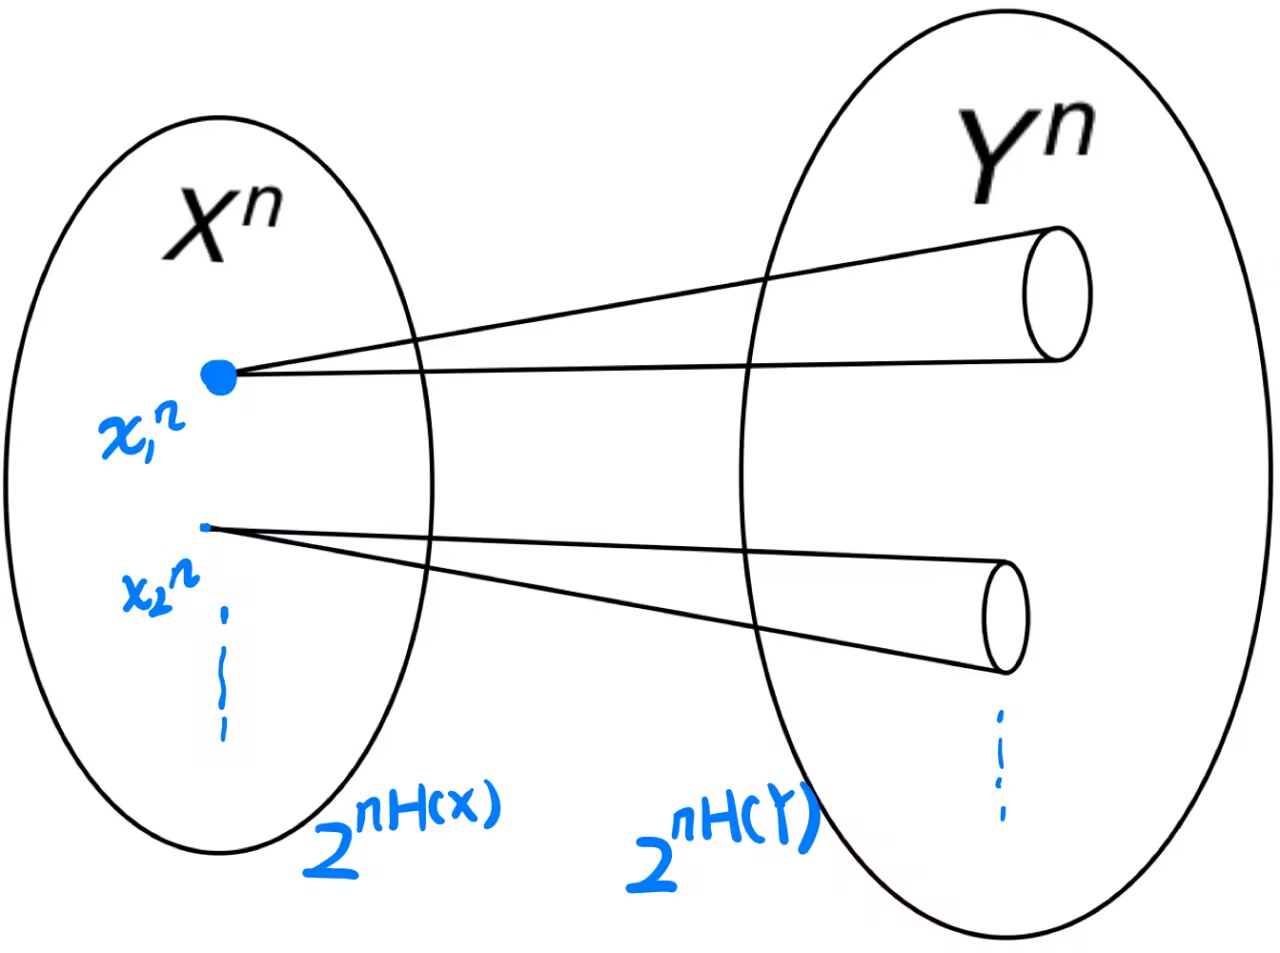
\includegraphics[width=0.5\textwidth]{./figures/chapter4/joint_typical_set.png}
\end{figure}

抽中一对$(x^n,y^n)$, 他们是联合典型的概率为 $\dfrac{2^{nH(X,Y)}}{2^{nH(X)}2^{nH(Y)}}=2^{-nI(X;Y)}$.

换一个角度: 对于每个$X^n$, 大约会有$\dfrac{2^{nH(X,Y)}}{2^{nH(X)}}=2^{nH(X|Y)}$个$Y^n$是与他联合典型的. 这样子每一个$Y^n$都会有一个$X^n$与他联合典型, 但是对于每一个$X^n$, 他会有$2^{nH(Y|X)}$个$Y^n$与他联合典型.
\end{proposition}